% Latex template: https://github.com/mqTeXUsers/Macquarie-University-Beamer-Theme

% Slide Masters:

% Title
% Text
% 2 column
% Full-image
% Bibliography
% Closing
 
\documentclass[aspectratio=1610, 11pt]{beamer} % Aspect ratio
% https://tex.stackexchange.com/a/14339/5483 
% Possible values: 1610, 169, 149, 54, 43 and 32.
% 169 = 16:9

\PassOptionsToPackage{table}{xcolor}    %https://tex.stackexchange.com/a/5365/5483

\usetheme{macquarie}
\usepackage{multicol} % https://tex.stackexchange.com/a/396018/5483
\usepackage{xurl}
\usepackage[british]{babel}       % Set language
% \usepackage[utf8x]{inputenc}      % Set encoding
\usepackage{colortbl}
\mode<presentation>           % Set options
{
  \usetheme{default}          % Set theme
  \usecolortheme{default}         % Set colors
  \usefonttheme{default}          % Set font theme
  \setbeamertemplate{caption}[numbered] % Set caption to be numbered
}

% Uncomment this to have the outline at the beginning of each section highlighted.
%\AtBeginSection[]
%{
%  \begin{frame}{Outline}
%    \tableofcontents[currentsection]
%  \end{frame}
%}

\usepackage{graphicx}         % For including figures
\usepackage{booktabs}         % For table rules
\usepackage{hyperref}         % For cross-referencing


\usepackage{enumitem} % https://tex.stackexchange.com/a/2292/5483

%https://tex.stackexchange.com/a/371844/5483
\setbeamerfont{bibliography entry author}{size=\tiny}
\setbeamerfont{bibliography entry title}{size=\tiny}
\setbeamerfont{bibliography entry location}{size=\tiny}
\setbeamerfont{bibliography entry note}{size=\tiny}
\setbeamerfont{bibliography item}{size=\tiny}

%https://tex.stackexchange.com/q/333587/5483
%TODO SHAWN REPLACE OSF URL
%\setbeamertemplate{footline}{\strut~\texttt{https://github.com/MQ-FOAR705/MQ-FOAR705-Week1}\hfill\insertframenumber~/~\inserttotalframenumber\strut~~~}

\title{FOAR705 Week 3} % Presentation title
\author{Brian Ballsun-Stanton | Shawn A Ross | Kathryn Elliot}               % Presentation author
\institute{Faculty of Arts}         % Author affiliation
\date{Friday 16 August 2019}                 % Today's date  
\begin{document}

% Title page
% This page includes the informations defined earlier including title, author/s, affiliation/s and the date
% \begin{frame}[noframenumbering]

\maketitle

  
% \end{frame}

\begin{frame}{Today's Plan}
  \tableofcontents
\end{frame}

\section{Minute card reflection}
\begin{frame}{Assignment overview 1}

One major theme of feedback (from sticky notes, slack, and the jargon document) is that we need to discuss all of the assignments and how they fit together.

\begin{itemize}[label=\textbullet]
\item Proof of Concept (Technology Demonstration)
\begin{itemize}[label=\textbullet]
% \item Scoping (Due sunday, because we misconfigured dates)
% \item Elaboration Plan: Finding tools and techniques that can help solve your problem. Due before class Week 4.
% \item Elaboration Results: Testing the claims of these tools and techniques. Do they do what they say they're going to do? Due before class week 6.
% \item Deployment: Design your proof of concept of your solution to the problem defined during your scoping? How will the tools and techniques you've found actually combine together to solve your problem? What do you need to do? (Week 9) -- Now, do it (week 11). 
% \item Testing and polishing. Make sure that there exists enough documentation and testing around your combination of tools and techniques such that other people might be able to use them somewhat reliably, \textit{or} document the known failings of your combination and articulate how, if given more time, you would proceed to fix them. (Week 13)
\item Scoping (due sunday)
\item Elaboration plan (due before class, week 4)
\item Elaboration results (due before class week 6)
\item Proof of Concept Design or starting `deployment' (Due before class week 7)
\item Proof of concept component demonstration (Due before class week 9)
\item Proof of concept linking demonstration (due before class week 11)
\item Final version (Due before class week 13)
\end{itemize}
\end{itemize}
\end{frame}

\begin{frame}{Assignment overview 2}
\begin{itemize}[label=\textbullet]

\item Learning Journal (Covered last week. Any technical work you do in this class should go into its own section). No formatting rules, though we disrecommend using word because it breaks things. (Due 4 times throughout semester)
\item Lighting Talks (PICO Presentations) (Presenting your Proof of Concept (Tech Demo)) in a 2 minute mixed presentation/poster format. See EGU Pico presentation. (During exam time)
\item Original Software Publication (Presenting your proof of concept as a paper which could be published in the SoftwareX Journal) (Due Week 13)
\end{itemize}

% Shawn, what visible thing will we change in reaction?
\end{frame}

\section{Jargon Busting}
\begin{frame}{To open with, some jargon busting}
Via @sheri: https://cloudstor.aarnet.edu.au/plus/f/3774955770

Some terms of note:

\begin{itemize}[label=\textbullet]
    \item Proof of Concept (POC): `Assignment for FOAR705. See "Scoping", "Elaboration", "Deployment" A mechanism for describing, then creating a technology (tool and/or technique) workflow to assist your research.' The major work you will be doing over this semester. 
    \item Typesetting: `Typesetting is the careful arrangement of text in a typeface in order to achieve maximum legibility,' \cite{Newcomb2019-hm}. The fourth step in the composition process (Preceded by Outlining (figuring out exactly what you want to say, and in what order, down to sub-paragraph detail), Writing, and Editing).
\end{itemize}


\end{frame}

\section{Data Carpentry}
\begin{frame}{Discussion from last week}

Discussion:

\begin{itemize}
\item Episode 1:
\begin{itemize}
\item What was wrong with the SAFI `messy' data?
\item What metadata should be recorded for the `clean' data?
\end{itemize}
\item Episode 2:
\begin{itemize}
\item What dirty data sets did you find?
\item What errors did you find counterintuitive?
\end{itemize}
\end{itemize}



\end{frame}
\begin{frame}{Dates as Data}

\begin{figure}[H]
        \centering
        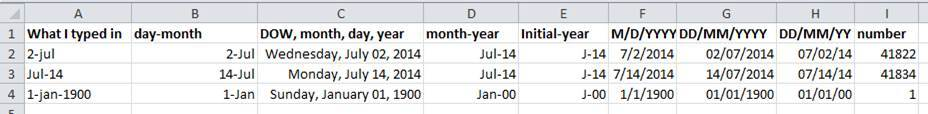
\includegraphics[width=\textwidth]{figures/excel_dates_1.jpg}
        \caption{Actual value in cells: `41822', `41834', and `1'. Dates as data, Data Carpentry. CC-By}
        \label{fig:bigdates}
    \end{figure}

Also beware: Regional Date formatting.


\end{frame}
\begin{frame}{Exercise}

Download and open the dates.xlsx file. This file contains a subset of the data from the SAFI interviews, including the dates on which the interviews were conducted.

Choose the tab of the spreadsheet that corresponds to the way you format dates in your location (either day first {\tt DD\_MM\_YEAR }, or month first {\tt MM\_DD\_YEAR} ).

Extract the components of the date to new columns. For this we can use the built in Excel functions:

{\tt =MONTH()} 

{\tt =DAY()}

{\tt =YEAR()}

Apply each of these formulas to its entire column. Make sure the new column is formatted as a number and not as a date.

\end{frame}

\begin{frame}{Exercise}
Using the same spreadsheet you used for the previous exercise, add another data point in the {\tt interview\_date} column by typing either {\tt 11/17} (if your location uses {\tt MM/DD} formatting) or {\tt 17/11} (if your location uses {\tt DD/MM} formatting). The {\tt Day}, {\tt Month}, and {\tt Year} columns should populate for this new data point. What year is shown in the {\tt Year} column?
\end{frame}

\begin{frame}{Notes on Quality Assurance}

\begin{itemize}[label=\textbullet]
    \item Do one thing at a time.
    \item Constrain inputs as much as you can.
    \item Calculations should have validation/sanity checks.
\end{itemize}
\end{frame}

\section{Computational Thinking}

\begin{frame}{What is Computational Thinking?}

Computers are good at some things. Mostly boring and repetitive things. 

People are good at other things. Mostly creative and interesting things.

Computers are fast but stupid. They need clear, step-by-step instructions (which they can then execute quickly).

Computational thinking is an approach that lets you decide \textbf{what} computers are good for, and \textbf{how} to tell the computer to do what you want.

\end{frame}

\begin{frame}{Decomposition and algorithm design}

\textbf{Computational Thinking }(CT) is a problem solving process that includes a number of characteristics and dispositions. \cite{Google2019-es}
\begin{itemize}[label=\textbullet]
    \item \textbf{Decomposition}: Breaking down data, processes, or problems into smaller, manageable parts.
    \item \textbf{Algorithm Design}: Developing the step by step instructions for solving this and similar problems.
\end{itemize}

Bonus points for:
\begin{itemize}
    \item \textbf{Pattern Recognition}: Observing patterns, trends, and regularities in data.
    \item \textbf{Abstraction}: Identifying the general principles that generate these patterns.
\end{itemize}
\end{frame}

\begin{frame}{Computational Thinking example}

'I need to produce properly formatted references and bibliography in my thesis'

[Articulate process in groups]

\end{frame}

 \section{Project management 101}

 \begin{frame}{Developing ideas towards a solution}
     So you have great ideas, what next? 
 \end{frame}

 \begin{frame}{Approach \#1: Top-down design (`Waterfall')}
  \begin{figure}[Waterfall]
     \centering
         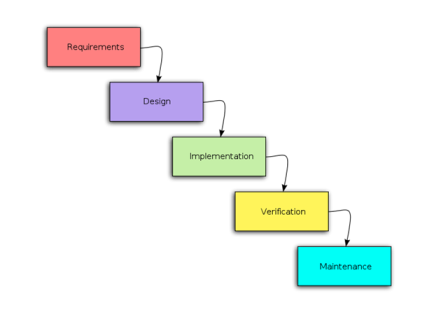
\includegraphics[height=.75\textheight]{figures/waterfall.png}
         \caption{Traditional and linear approach \cite{Parody2018-if}} 
         \label{fig:6}
  \end{figure}
 \end{frame}

 \begin{frame}{Approach \#2: Iterative design with course corrections (`Agile')}
  \begin{figure}[Agile]
     \centering
         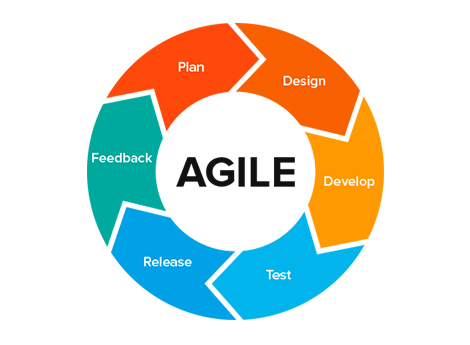
\includegraphics[height=.75\textheight]{figures/agile.png}
         \caption{Design-test-repeat approach to PM \cite{Parody2018-if}} 
         \label{fig:7}
  \end{figure}
 \end{frame}

 \begin{frame}{Manifesto for Agile Software Development}
 We are uncovering better ways of developing software by doing it and helping others do it. Through this work we have come to value:
     \begin{itemize}[label=\textbullet]
         \item \textbf{Individuals and interactions} over processes and tools
         \item \textbf{Working software} over comprehensive documentation
         \item \textbf{Customer collaboration} over contract negotiation
         \item \textbf{Responding to change} over following a plan
     \end{itemize}
 That is, while there is value in the items on the right, we value the items on the left more. \cite{Atlassian2019-xl}
 \end{frame}

 \begin{frame}{Tool \#1: Gantt chart}
  \begin{figure}[Gantt]
     \centering
         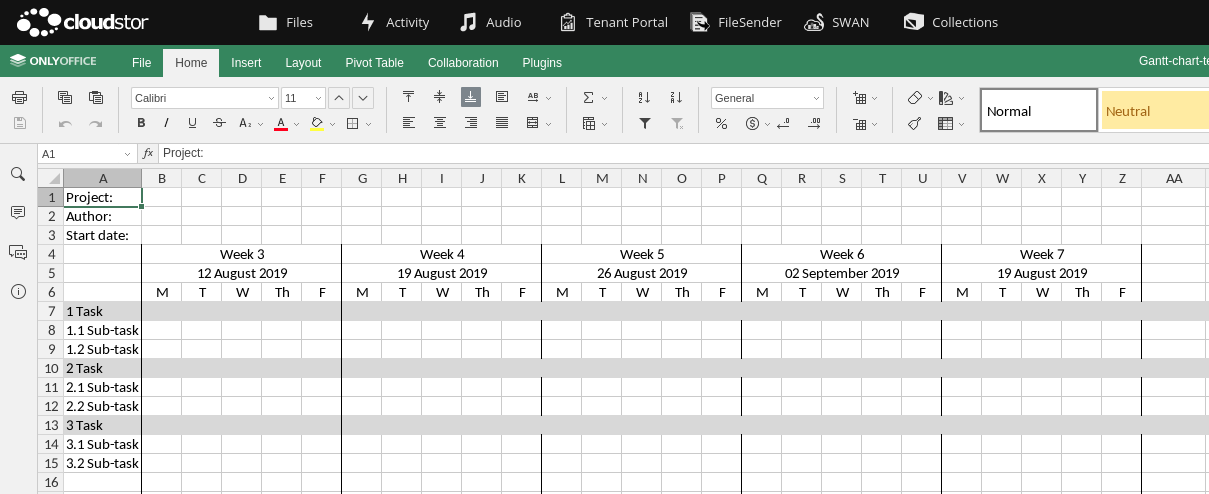
\includegraphics[height=.75\textheight]{figures/gantt.png}
         \caption{A Gantt Chart template (on Cloudstor)}
         \label{fig:8}
  \end{figure}
 \end{frame}

 \begin{frame}{Tool \#2: Kanban board}
  \begin{figure}[Kanban]
     \centering
         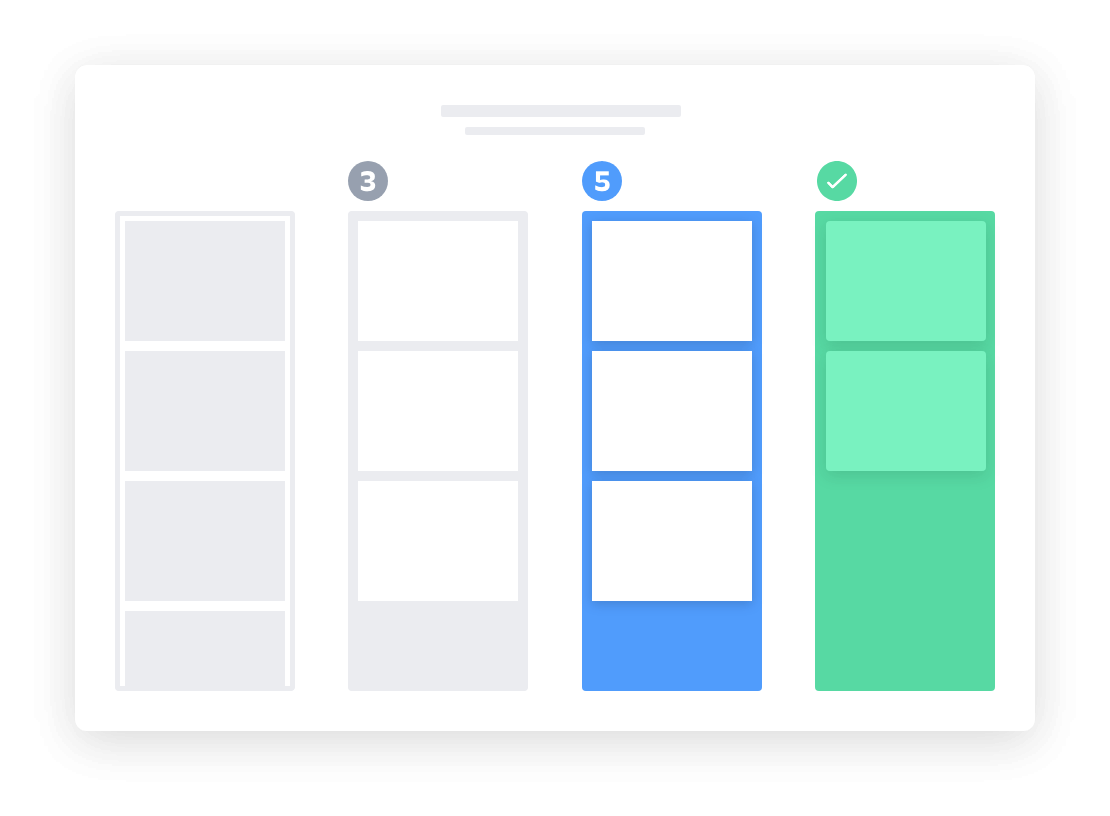
\includegraphics[height=.75\textheight]{figures/kanban.png}
         \caption{Schematic Kanban board \cite{Atlassian2019-bo}}
         \label{fig:9}
  \end{figure}
 \end{frame}

 \begin{frame}{A Kanban board should}
     \begin{itemize}[label=\textbullet]
         \item Visualise your work
         \item Limit work in progress
     \end{itemize}
 Kanban boards often have columns like: Backlog (wish list), To do, In progress, Done, with the 'To do' and 'In progress' columns having work limits (e.g., 3-5 tasks). 

 Trello is a popular application for Kanban. Atlassian has Kanban learning materials online \cite{Atlassian2019-bo}.
 \end{frame}

% %  Outline
% % This page includes the outline (Table of content) of the presentation. All sections and subsections will appear in the outline by default.
% % \begin{frame}{The context of Research Data Management}
% %   \tableofcontents
% % \end{frame}

% % % The following is the most frequently used slide types in beamer
% % % The slide structure is as follows:
% % %
% % %\begin{frame}{<slide-title>}
% % % <content>
% % %\end{frame}

% % \section{Code of Conduct}

% % \begin{frame}{Unit Code of Conduct}
% % This class is using a great deal of material from The Carpentries. All interactions related to this class, inside and outside, abide by The Carpentries Code of Conduct.

% % Report code of conduct violations to Shawn, Brian, or eresearch@mq.edu.au.

% % \url{https://docs.carpentries.org/topic\_folders/policies/code-of-conduct.html}

% % In summary, we want to emphasise:

% % \begin{itemize}[label=\textbullet]
% %     \item Use welcoming and inclusive language
% %     \item Be respectful of different viewpoints and experiences
% %     \item Gracefully accept constructive criticism
% %     \item Focus on what is best for the community
% %     \item Show courtesy and respect towards other community members
% % \end{itemize}

% % \end{frame}

% % \section{Expectations}

% % \begin{frame}{Is the content 'too hard'?}
% %  `I still have my concerns about how over-technical this course is given it is now meant to be taken by students from across the entire Faculty from diverse backgrounds and with diverse interests...I suspect will cause students anxiety and maybe lead to drop out.'
% %     \begin{itemize}[label=\textbullet]
% %         \item Before we start, what was your reaction to reading the Unit description?
% %         \item Do you agree with the quote above?
% %     \end{itemize}
% % \end{frame}

% % \begin{frame}{Expectations and workload}
% %   You are undertaking an Masters of Research at a top one-percent university (QS ranking 125 in Arts and Humanities, 202 in Social Sciences). Expectations and workload higher than what you are accustomed to.
% %     \begin{itemize}[label=\textbullet]
% %         \item Expect a workload of six hours per week outside of class to earn a DN or HD.
% %         \item Avoid missing classes. If you do, expect to spend four hours to catch up.
% %         \item If you want to continue to a PhD you need to maintain a DN or HD average.
% %         \item Both of us have taught overseas and are engaged with international trends in research technology. This unit has been calibrated to the international environment.
% %         \item Considering the academic job market, competition is fierce.
% %         \item Most of you will not get academic jobs, so transferable skills are crucial.
% %         \item It is our job to prepare you for this environment, and yours to make yourself competitive.
% %     \end{itemize}
% % \end{frame}

% % \begin{frame}{Assessment}

% % \begin{itemize}[label=\textbullet]
% %     \item Proof of Concept
% %     \item Original Software Publication
% %     \item Lightning talk
% %     \item Learning journal
% % \end{itemize}

% % \end{frame}

% % \section{Don't panic!}

% % \begin{frame}{Data Carpentry: a proven approach}
% %     `Building communities teaching universal data literacy'
       
% %     `Data Carpentry trains researchers in the core data skills for efficient, shareable, and reproducible research practices. We run accessible, inclusive training workshops; teach openly available, high-quality, domain-tailored lessons; and foster an active, inclusive, diverse instructor community that promotes and models reproducible research as a community norm.' \cite{Teal2016-gy}

% %     `Since 1998, Software Carpentry has been teaching researchers the computing skills they need to get more done in less time and with less pain. Our volunteer instructors have run hundreds of events for more than 34,000 researchers since 2012.' \cite{Duckles2018-fu}
% % \end{frame}

% % \begin{frame}{Data Carpentry: widely used worldwide in HASS}
% %     Carpentries training is used all over the world to teach digital literacy and computational thinking to Humanities and Social Sciences students and researchers.
% %     \begin{itemize}[label=\textbullet]
% %         \item Digital Humanities at Oxford Summer School
% %         \item CODATA-RDA School of Research Data Science
% %         \item Australian Research Data Cloud training
% %         \item THATCamps (e.g., at Sydney ResBaz 2019)
% %     \end{itemize}
% % \end{frame}

% % \begin{frame}{Data Carpentry: used at Macquarie}
% %   Other MRes students at this university have successfully undergone DC training:
% %     \begin{itemize}[label=\textbullet]
% %         \item BIOL703 Research Skills for Biology
% %         \item No excess attrition, high student satisfaction, good feedback
% %         \item Nominated for a Vice-Chancellor's Learning and Teaching award
% %         \item Is the background or needs of Arts students that different from ecology, biology, environmental sciences, and related fields?
% %     \end{itemize}
% % \end{frame}

% % \begin{frame}{Previous HASS MRes students have thrived}
% %   \url{https://www.youtube.com/watch?v=r9jpe9\_2z3c}
% % \end{frame}

% % \section{What, and why?}

% % \begin{frame}{Digital literacy: creators, not consumers}
% %     \begin{figure}[H]
% %         \centering
% %         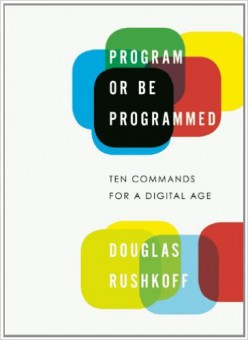
\includegraphics[height=.6\textheight]{figures/2011-ProgOrBeProgged-248x340.jpg}
% %         \caption{Program or be Programmed, Douglas Rushkoff}
% %         \label{fig:programmed}
% %     \end{figure}
  
% %   See also: \url{https://impossiblehq.com/an-unexpected-ass-kicking/}
% % %insert 'Program or be programmed' book cover image, and link to 'An unexpected ass kicking' %https://rushkoff.com/books/program-or-be-programmed/
% % %https://impossiblehq.com/an-unexpected-ass-kicking/

% % \end{frame}

% % \begin{frame}{Computational thinking: what can you do with a computer?}
% % \begin{figure}[H]
% %         \centering
% %         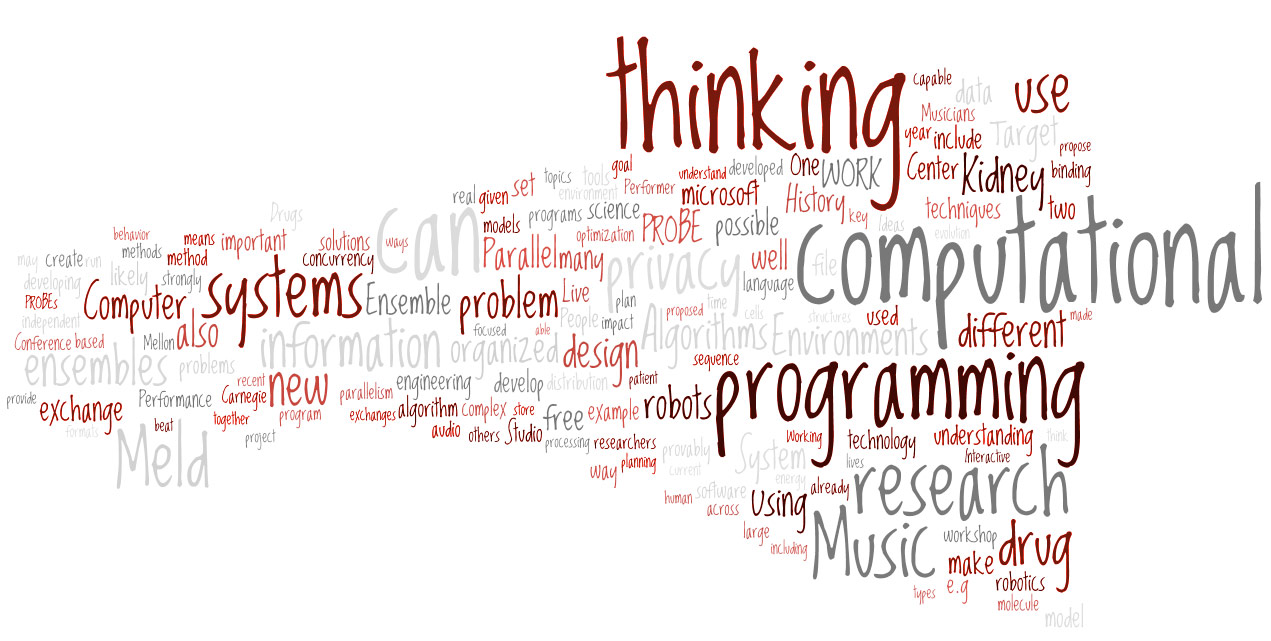
\includegraphics[height=.6\textheight]{figures/ctc-w2b.jpg}
% %         \caption{'To flourish in today's world, computational thinking has to be a fundamental part of the way people think and understand the world.' \cite{Center\_for\_Computational\_Thinking2012-tt}}
% %         \label{fig:ctc}
% %     \end{figure}
% % %insert https://www.cs.cmu.edu/~CompThink/images/ctc-w2b.jpg
% % %caption: 'To flourish in today's world, computational thinking has to be a fundamental part of the way people think and understand the world.' https://www.cs.cmu.edu/~CompThink/

% % \end{frame}

% % \begin{frame}{Tools and approaches}
% % Only within these frameworks can you use available tools and approaches - but we will introduce you to a range of them, customised to the disciplinary mix in the class.
% %     \begin{itemize}[label=\textbullet]
% %         \item Research design and project management
% %         \item Data management planning
% %         \item Data capture
% %         \item Data analysis and collaboration
% %         \item Data archiving and dissemination
% %     \end{itemize}

% % \end{frame}


% % \section{Tools and Communication}
% % \begin{frame}{Discussion on which tools we will use as a class}

% % \begin{itemize}[label=\textbullet]
% %     \item Chat/coordination/project management software
% %     \item Typesetting software
% %     \item Version control online repository
% %     \item File sharing mechanisms
% %     \item Backup mechanisms
% % \end{itemize}

% % \end{frame}

% % \begin{frame}{Coordination outside of class}

% % \begin{itemize}[label=\textbullet]
% %     \item Hacky-hour/study groups: \url{https://science.mozilla.org/programs/studygroups}
% %     \item Consultation Hours: Friday 12:45-1:45pm (AHH Level 2 lobby) and 4:15-5:15pm, campus hub (before and after seminar)
% %     \item \url{https://twitter.com/Rusers\_MQ}
% % \end{itemize}

% % \end{frame}

% % \section{Moving on to Data Carpentry}


% % \begin{frame}{Pre-Carpentry survey}

% % At the start and end of every carpentries workshop, we poll participants.

% % \url{https://bit.ly/FOAR705-pre}

% % \begin{figure}[H]
% %         \centering
% %         
\includegraphics[height=.6\textheight]{figures/qr.jpeg}
% %         \caption{\url{https://mqedu.qualtrics.com/jfe/form/SV\_5v6iQJSBZDNhq4d?workshop=FOAR705-2019}}
% %         \label{fig:foarqr}
% %     \end{figure}
    
% % \end{frame}

% % \begin{frame}{Sticky notes}

% % We use sticky notes during our workshops (and thus during our classes) to indicate progress or needs for assistance. 

% % We also use them as minute cards for feedback and the end of each session. 

% % \end{frame}
% % \begin{frame}{Starting the workshop}
% %     \begin{itemize}
% %         \item \url{https://datacarpentry.org/socialsci-workshop/}
% %         \item \url{https://datacarpentry.org/spreadsheets-socialsci/setup.html}
% %         \item \url{https://datacarpentry.org/openrefine-socialsci/setup.html}
% %         \item \url{https://datacarpentry.org/r-socialsci/setup.html}
% %     \end{itemize}
% % \end{frame}


% % % \bibliographystyle{apalike}

% % % Adding the option 'allowframebreaks' allows the contents of the slide to be expanded in more than one slide.
% % % The "1" comes from the outer theme"


\section{Minute cards!}
\begin{frame}{Feedback time}

On your green sticky, write one thing we did well today.

On your red sticky, write one thing we could improve upon for next time. Be specific. 

\end{frame}

\section{References}

\begin{multicols}{2}[]
\bibliography{references}
\bibliographystyle{apalike}
\end{multicols}


% \begin{frame}[allowframebreaks]{References}
  
%   \bibliography{references}
%   \bibliographystyle{apalike}
% \end{frame}


\begin{frame}{Thank you!}

% This presentation is available at:
% \texttt{https://osf.io/...}

Source code for this presentation is available at: \url{https://github.com/MQ-FOAR705/MQ-FOAR705-Week3}

This work is licensed under a Creative Commons Attribution 4.0 International License.

\end{frame}



\end{document}